\documentclass[11pt]{article}

\usepackage[margin=1in]{geometry}
\usepackage{amsmath,amssymb,amsthm,mathtools}
\usepackage{enumitem}
\usepackage{booktabs}
\usepackage{tikz}
\usetikzlibrary{arrows.meta,positioning}
\usepackage{ytableau}
\usepackage[colorlinks=true,linkcolor=blue!50!black]{hyperref}

% ------------------------------------------------------------------
% Theorem environments
% ------------------------------------------------------------------
\newtheorem{theorem}{Theorem}[section]
\newtheorem{lemma}[theorem]{Lemma}
\newtheorem{corollary}[theorem]{Corollary}
\theoremstyle{definition}
\newtheorem{definition}[theorem]{Definition}
\newtheorem{example}[theorem]{Example}
\newtheorem{convention}[theorem]{Convention}
\theoremstyle{remark}
\newtheorem{remark}[theorem]{Remark}

% ------------------------------------------------------------------
% Macros
% ------------------------------------------------------------------
\newcommand{\C}{\mathbb{C}}
\DeclareMathOperator{\Irr}{Irr}
\DeclareMathOperator{\Res}{Res}
\DeclareMathOperator{\Hom}{Hom}
\DeclareMathOperator{\End}{End}
\DeclareMathOperator{\im}{im}
\DeclareMathOperator{\pth}{path}   % path(W,V): paths from W to V
\DeclareMathOperator{\Pth}{Path}   % Path(V) = path(C_triv, V)
\newcommand{\Ctriv}{\C_{\mathrm{triv}}}
\newcommand{\Csgn}{\C_{\mathrm{sgn}}}
\newcommand{\h}{h}                 % standard representation h^n
\newcommand{\into}{\hookrightarrow}

\ytableausetup{boxsize=1.35em,centertableaux}

\title{Representations of the Symmetric Group:\\
the Branching Graph, Paths, and the Gelfand--Tsetlin Basis}
\author{}
\date{}

\begin{document}
\maketitle

% ==================================================================
\section{Setup and notation}
% ==================================================================

Throughout, representations are finite-dimensional over $\C$. For each
$n\ge 1$ we regard $S_{n-1}\subset S_n$ as the permutations fixing $n$, which
gives a chain
\[
  S_1\subset S_2\subset S_3\subset\cdots .
\]
For $m\le n$ we write $\Res^{S_n}_{S_m}$ for restriction from $S_n$ to $S_m$.
$\Irr(S_n)$ denotes the set of (isomorphism classes of) irreducible
representations of $S_n$; these are indexed by partitions $\lambda\vdash n$,
and we write $V^\lambda$ for the irreducible representation attached to
$\lambda$.

\paragraph{Some irreducible representations.}
\begin{itemize}[nosep]
  \item $\Ctriv$: the trivial representation; $\Csgn$: the sign representation.
  \item $\h^n=\{x\in\C^n : x_1+\cdots+x_n=0\}$: the standard representation of
        $S_n$, of dimension $n-1$ ($\h^n\cong V^{(n-1,1)}$).
  \item $\Irr(S_1)=\{\Ctriv\}$ and $\Irr(S_2)=\{\Ctriv,\Csgn\}$.
\end{itemize}

\paragraph{Jucys--Murphy elements.}
For $k\ge 1$ put
\[
  J_k \;=\; (1\,k)+(2\,k)+\cdots+(k-1\;k)\;\in\;\C[S_k],
  \qquad (J_1=0).
\]
\begin{lemma}\label{lem:JM-commute}
$J_k$ commutes with every element of $\C[S_{k-1}]$.
\end{lemma}
\begin{proof}
For $\sigma\in S_{k-1}$ we have $\sigma(i\,k)\sigma^{-1}=(\sigma(i)\,k)$, and
$\sigma$ permutes $\{1,\dots,k-1\}$. Hence $\sigma J_k\sigma^{-1}=J_k$.
\end{proof}

\begin{theorem}[Branching rule]\label{thm:branching}
For $\lambda\vdash n$,
\[
  \Res^{S_n}_{S_{n-1}} V^\lambda \;\cong\;
  \bigoplus_{\substack{\mu\vdash n-1\\ \lambda/\mu \text{ is one box}}} V^\mu .
\]
In particular, $\Res^{S_n}_{S_{n-1}}V^\lambda$ is multiplicity-free.
\end{theorem}

\begin{corollary}\label{cor:mult-free}
Let $V\in\Irr(S_n)$ and $U\in\Irr(S_{n-1})$. Then
$\dim\Hom_{S_{n-1}}\!\bigl(U,\Res^{S_n}_{S_{n-1}}V\bigr)\in\{0,1\}$. If it is
$1$, then
\[
  \Hom_{S_{n-1}}\!\bigl(U,\Res^{S_n}_{S_{n-1}}V\bigr)\cong\C,
\]
so any two inclusions $U\into V$ agree up to a scalar in $\C^\times$. In
particular they all have the same image, namely the $U$-isotypic component
of $\Res^{S_n}_{S_{n-1}}V$.
\end{corollary}

\begin{lemma}\label{lem:JM-scalar}
Let $V\in\Irr(S_k)$, $U\in\Irr(S_{k-1})$ with $U\into\Res^{S_k}_{S_{k-1}}V$,
and let $U'\subseteq V$ be the image. Then $J_k$ preserves $U'$ and acts on it
by a scalar.
\end{lemma}
\begin{proof}
By Lemma~\ref{lem:JM-commute}, $J_k\colon V\to V$ is
$S_{k-1}$-equivariant, so it preserves each $S_{k-1}$-isotypic component. By
Corollary~\ref{cor:mult-free}, $U'$ is the $U$-isotypic component and is
irreducible, so $J_k|_{U'}\in\End_{S_{k-1}}(U')=\C$ by Schur's lemma.
\end{proof}

% ==================================================================
\section{The branching graph}
% ==================================================================

\begin{definition}
The \emph{branching graph} of $S_1\subset S_2\subset\cdots$ is the directed
graph with
\begin{itemize}[nosep]
  \item vertices: $\displaystyle\bigsqcup_{n\ge1}\Irr(S_n)$;
  \item edges: for $V\in\Irr(S_n)$ and $U\in\Irr(S_{n-1})$,
  \[
    V\longleftarrow U
    \quad\iff\quad
    \Hom_{S_{n-1}}\!\bigl(U,\Res^{S_n}_{S_{n-1}}(V)\bigr)\neq 0 .
  \]
\end{itemize}
We label the edge $U\to V$ by the scalar by which $J_n$ acts on the image of
$U$ in $V$ (well defined by Corollary~\ref{cor:mult-free} and
Lemma~\ref{lem:JM-scalar}).
\end{definition}

By the branching rule, the vertices on level $n$ are the Young diagrams with
$n$ boxes, and $U\to V$ is an edge exactly when the diagram of $V$ is obtained
from that of $U$ by adding one box.

\begin{example}[From $\h^4$ down to $S_1$]\label{ex:h4}
Restricting step by step:
\[
  \h^4
  \;\xrightarrow{\ \Res^{S_4}_{S_3}\ }\;
  \underbrace{\h^3}_{J_4=+2}\oplus\underbrace{\Ctriv}_{J_4=-1}
  \;\xrightarrow{\ \Res^{S_3}_{S_2}\ }\;
  \underbrace{\Csgn}_{J_3=+1}\oplus\underbrace{\Ctriv}_{J_3=-1}
  \;\oplus\;\underbrace{\Ctriv}_{J_3=+2},
\]
where the first two summands on the right come from $\h^3$ and the last one
from $\Ctriv$. Finally $J_2=(1\,2)$ acts by $-1$ on $\Csgn$ and by $+1$ on
$\Ctriv$.

\smallskip
\noindent\emph{Check.} In $\h^4$, the vector $(1,1,1,-3)$ spans the copy of
$\Ctriv$ for $S_3$ and $(1,-1,0,0)$ lies in the copy of $\h^3$; one computes
\[
  J_4(1,1,1,-3)=(-1,-1,-1,3)=-(1,1,1,-3),\qquad
  J_4(1,-1,0,0)=(2,-2,0,0)=2\,(1,-1,0,0).
\]
In $\h^3$, the vector $(1,-1,0)$ spans $\Csgn$ and $(1,1,-2)$ spans $\Ctriv$
for $S_2$, and
\[
  J_3(1,-1,0)=(1,-1,0),\qquad J_3(1,1,-2)=-(1,1,-2).
\]
On $\Ctriv$ of $S_3$, $J_3$ acts by $2$.

The part of the branching graph lying below $\h^4$ is shown in
Figure~\ref{fig:branching}, once with representations and once with Young
diagrams (each box filled with its content, see
Remark~\ref{rem:content}).
\end{example}

\begin{figure}[ht]
\centering
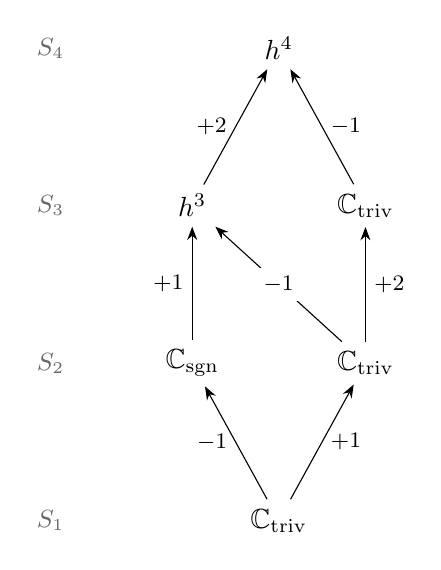
\begin{tikzpicture}[
    >=Stealth,
    lbl/.style={font=\footnotesize, inner sep=3pt},
    lvl/.style={font=\small, text=black!60}]
  % level labels
  \node[lvl] at (-2.4,6) {$S_4$};
  \node[lvl] at (-2.4,4) {$S_3$};
  \node[lvl] at (-2.4,2) {$S_2$};
  \node[lvl] at (-2.4,0) {$S_1$};
  % vertices
  \node (h4) at (0.5,6) {$\h^4$};
  \node (h3) at (-0.6,4) {$\h^3$};
  \node (t3) at (1.6,4) {$\Ctriv$};
  \node (s2) at (-0.6,2) {$\Csgn$};
  \node (t2) at (1.6,2) {$\Ctriv$};
  \node (t1) at (0.5,0) {$\Ctriv$};
  % edges U -> V (arrows point up)
  \draw[->] (h3) -- node[lbl,left]  {$+2$} (h4);
  \draw[->] (t3) -- node[lbl,right] {$-1$} (h4);
  \draw[->] (s2) -- node[lbl,left]  {$+1$} (h3);
  \draw[->] (t2) -- node[lbl,fill=white,pos=0.5] {$-1$} (h3);
  \draw[->] (t2) -- node[lbl,right] {$+2$} (t3);
  \draw[->] (t1) -- node[lbl,left]  {$-1$} (s2);
  \draw[->] (t1) -- node[lbl,right] {$+1$} (t2);
\end{tikzpicture}
\hspace{2.5cm}
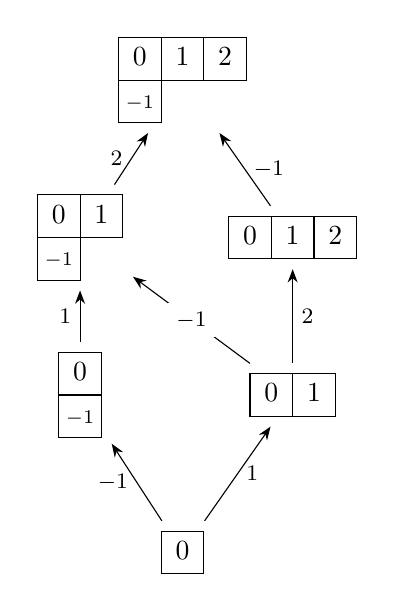
\begin{tikzpicture}[
    >=Stealth,
    lbl/.style={font=\footnotesize, inner sep=3pt}]
  \node (a4) at (0.5,6)  {\begin{ytableau} 0 & 1 & 2 \\ \scriptstyle -1 \end{ytableau}};
  \node (a3) at (-0.8,4) {\begin{ytableau} 0 & 1 \\ \scriptstyle -1 \end{ytableau}};
  \node (b3) at (1.9,4)  {\begin{ytableau} 0 & 1 & 2 \end{ytableau}};
  \node (a2) at (-0.8,2) {\begin{ytableau} 0 \\ \scriptstyle -1 \end{ytableau}};
  \node (b2) at (1.9,2)  {\begin{ytableau} 0 & 1 \end{ytableau}};
  \node (a1) at (0.5,0)  {\begin{ytableau} 0 \end{ytableau}};
  \draw[->] (a3) -- node[lbl,left]  {$2$}  (a4);
  \draw[->] (b3) -- node[lbl,right] {$-1$} (a4);
  \draw[->] (a2) -- node[lbl,left]  {$1$}  (a3);
  \draw[->] (b2) -- node[lbl,fill=white,pos=0.5] {$-1$} (a3);
  \draw[->] (b2) -- node[lbl,right] {$2$}  (b3);
  \draw[->] (a1) -- node[lbl,left]  {$-1$} (a2);
  \draw[->] (a1) -- node[lbl,right] {$1$}  (b2);
\end{tikzpicture}
\caption{The part of the branching graph below $\h^4$. An edge $U\to V$ is
labelled by the eigenvalue of $J_n$ on the copy of $U$ inside $V$. Right: the
same graph with Young diagrams; the label of each edge is the content of the
box that is added.}
\label{fig:branching}
\end{figure}

% ==================================================================
\section{Paths}
% ==================================================================

\begin{definition}
Let $m\le n$, $W\in\Irr(S_m)$, $V\in\Irr(S_n)$. Set
\[
  \pth(W,V)=\{\text{paths in the branching graph from $W$ to $V$}\},
\]
i.e.\ sequences $p=(W=V^m\to V^{m+1}\to\cdots\to V^n=V)$ with
$V^k\in\Irr(S_k)$ and each $V^{k-1}\to V^k$ an edge.
\end{definition}

\noindent\emph{Note} (case $m=1$): $\Irr(S_1)=\{\Ctriv\}$, so every path that
starts on level $1$ starts at $\Ctriv$.

\begin{definition}
For $V\in\Irr(S_n)$,
\[
  \Pth(V)=\pth(\Ctriv,V)\qquad(\Ctriv\in\Irr S_1,\ V\in\Irr S_n),
  \qquad
  \Pth_n=\bigsqcup_{V\in\Irr(S_n)}\Pth(V).
\]
\end{definition}

\begin{convention}[Choice of embeddings]
Recall: if $V\leftarrow U$ is an edge with $V\in\Irr(S_n)$,
$U\in\Irr(S_{n-1})$, then
$\Hom_{S_{n-1}}(U,V|_{S_{n-1}})\cong\C$ (Corollary~\ref{cor:mult-free}), so
any two inclusions $U\into V$ are the same up to scalars in $\C^\times$. Fix
once and for all, for every edge $U\to V$, an $S_{n-1}$-equivariant inclusion
$\iota_{U,V}\colon U\into V$.
\end{convention}

\begin{definition}
For a path $p=(V^m\to V^{m+1}\to\cdots\to V^n)\in\pth(V^m,V^n)$ let
\[
  \varphi_p=\iota_{V^{n-1},V^n}\circ\cdots\circ\iota_{V^m,V^{m+1}}
  \colon\;
  V^m\into V^{m+1}\into V^{m+2}\into\cdots\into V^n ,
\]
\[
  V^m(p)=\im(\varphi_p)\subseteq V^n .
\]
Each $\iota_{V^{k-1},V^k}$ is $S_{k-1}$-equivariant, hence
$S_m$-equivariant, so $\varphi_p$ is an injective $S_m$-homomorphism
$V^m\to\Res^{S_n}_{S_m}V^n$ and $V^m(p)\cong V^m$ is an $S_m$-subrepresentation
of $V^n$. Changing the choices of the $\iota$'s rescales $\varphi_p$ by an
element of $\C^\times$, so $V^m(p)$ does not depend on them.
\end{definition}

\begin{theorem}\label{thm:res}
\[
  \Res^{S_n}_{S_m}V^n \;=\;
  \bigoplus_{W\in\Irr(S_m)}\ \bigoplus_{p\in\pth(W,V^n)} W(p)
  \qquad\text{(internal direct sum).}
\]
In particular, the multiplicity of $W$ in $\Res^{S_n}_{S_m}V^n$ equals
$|\pth(W,V^n)|$.
\end{theorem}

\begin{proof}
Repeated use of the branching rule; formally, induction on $n-m$. The case
$n=m$ is trivial. For $n>m$, Theorem~\ref{thm:branching} and
Corollary~\ref{cor:mult-free} give an internal decomposition into isotypic
components
\[
  \Res^{S_n}_{S_{n-1}}V^n=\bigoplus_{U\to V^n}\iota_{U,V^n}(U).
\]
By induction, for each such $U$ we have
$\Res^{S_{n-1}}_{S_m}U=\bigoplus_{W}\bigoplus_{q\in\pth(W,U)}W(q)$ inside $U$.
Applying the injective $S_m$-map $\iota_{U,V^n}$ preserves this direct sum,
and $\iota_{U,V^n}(W(q))=W(q')$ where $q'$ is $q$ followed by the edge
$U\to V^n$. Since every path from $W$ to $V^n$ arises in exactly one way like
this (from its last edge), the claim follows.
\end{proof}

% ==================================================================
\section{Weights of paths}
% ==================================================================

\begin{definition}
Let $p=(V^m\to\cdots\to V^n)\in\pth(V^m,V^n)$. For $k=m+1,\dots,n$ let
$\omega_k\in\C$ be the scalar by which $J_k$ acts on the image of $V^{k-1}$ in
$V^k$ (Lemma~\ref{lem:JM-scalar}), i.e.\ the label of the edge
$V^{k-1}\to V^k$. The \emph{weight} of $p$ is
\[
  \omega_p=(\omega_{m+1},\dots,\omega_n)\in\C^{\,n-m}.
\]
\end{definition}

\begin{example}\leavevmode
\begin{enumerate}[nosep]
  \item $p=(\Ctriv\to\Ctriv)$, from $S_1$ to $S_2$: $J_2=(1\,2)$ acts on
        $\Ctriv$ by $+1$, so $\omega_p=(1)$.
  \item $p=(\Ctriv\to\Csgn)$: $J_2$ acts by $-1$, so $\omega_p=(-1)$.
  \item $p=(\Ctriv\to\Csgn\to\h^3)\in\Pth(\h^3)$:
\[
  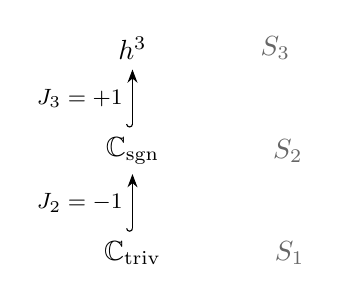
\begin{tikzpicture}[>=Stealth, baseline=(m.base)]
    \node (c1) at (0,0)   {$\Ctriv$};
    \node (m)  at (0,1.3) {$\Csgn$};
    \node (c3) at (0,2.6) {$\h^3$};
    \draw[{Hooks[right]}->] (c1) -- node[left,font=\footnotesize]{$J_2=-1$} (m);
    \draw[{Hooks[right]}->] (m)  -- node[left,font=\footnotesize]{$J_3=+1$} (c3);
    \node[right=1.2cm of c1, text=black!60] {$S_1$};
    \node[right=1.2cm of m,  text=black!60] {$S_2$};
    \node[right=1.2cm of c3, text=black!60] {$S_3$};
  \end{tikzpicture}
  \qquad\qquad \omega_p=(-1,\,1).
\]
  \item From Figure~\ref{fig:branching}, the three elements of $\Pth(\h^4)$
        and their weights $(\omega_2,\omega_3,\omega_4)$ are:
\[
  \begin{array}{ll}
    \toprule
    p & \omega_p\\
    \midrule
    \Ctriv\to\Csgn\to\h^3\to\h^4   & (-1,\ 1,\ 2)\\
    \Ctriv\to\Ctriv\to\h^3\to\h^4  & (1,\ -1,\ 2)\\
    \Ctriv\to\Ctriv\to\Ctriv\to\h^4 & (1,\ 2,\ -1)\\
    \bottomrule
  \end{array}
\]
\end{enumerate}
\end{example}

% ==================================================================
\section{A basis of \texorpdfstring{$\Hom_{S_m}(V^m,\Res^{S_n}_{S_m}V^n)$}{Hom(V\^{}m, Res V\^{}n)}}
% ==================================================================

For $k>m$ we have $S_m\subseteq S_{k-1}$, so $J_k$ commutes with $\C[S_m]$
(Lemma~\ref{lem:JM-commute}). Hence $J_k$ acts on
$\Hom_{S_m}(V^m,\Res^{S_n}_{S_m}V^n)$ by
\[
  (J_k\cdot\varphi)(w)=J_k\cdot\varphi(w)\qquad(w\in V^m).
\]

\begin{lemma}\label{lem:basis}
Let $V^m\in\Irr(S_m)$, $V^n\in\Irr(S_n)$.
\begin{enumerate}[label=(\alph*),nosep]
  \item $\{\varphi_p\}_{p\in\pth(V^m,V^n)}$ is a basis of
        $\Hom_{S_m}\!\bigl(V^m,\Res^{S_n}_{S_m}(V^n)\bigr)$.
  \item Each $\varphi_Q$ is an eigenvector of $J_k$ for
        $k\in\{m+1,\dots,n\}$: $J_k\cdot\varphi_Q=\omega_k\,\varphi_Q$, where
        $\omega_Q=(\omega_{m+1},\dots,\omega_n)$.
\end{enumerate}
\end{lemma}

\begin{proof}
(a) \emph{Basis.} By Theorem~\ref{thm:res},
\[
  \Res^{S_n}_{S_m}(V^n)=\bigoplus_{W\in\Irr(S_m)}\ \bigoplus_{Q\in\pth(W,V^n)}W(Q),
\]
hence
\begin{align*}
  \Hom_{S_m}\!\bigl(V^m,\Res^{S_n}_{S_m}V^n\bigr)
  &\cong\bigoplus_{W\in\Irr(S_m)}\ \bigoplus_{Q\in\pth(W,V^n)}
     \Hom_{S_m}\!\bigl(V^m,W(Q)\bigr)\\
  &=\bigoplus_{Q\in\pth(V^m,V^n)}\Hom_{S_m}\!\bigl(V^m,V^m(Q)\bigr),
\end{align*}
because $W(Q)\cong W$ is irreducible, so by Schur's lemma the summand vanishes
unless $W=V^m$. For $W=V^m$ the summand is one-dimensional and spanned by the
isomorphism $\varphi_Q\colon V^m\to V^m(Q)$. So the right-hand side has basis
$\{\varphi_Q\}_{Q\in\pth(V^m,V^n)}$.

\smallskip
(b) \emph{Eigenvalue.} Let $k\in\{m+1,\dots,n\}$ and
$Q=(V^m\to\cdots\to V^n)$. Factor
\[
  \varphi_Q=\psi\circ\iota_{V^{k-1},V^k}\circ\chi,
  \qquad
  \chi\colon V^m\into V^{k-1},\quad
  \psi\colon V^k\into V^n,
\]
where $\chi$ and $\psi$ are the composites of the inclusions along the first
and last parts of $Q$. Every inclusion in $\psi$ is $S_j$-equivariant for some
$j\ge k$, so $\psi$ is $S_k$-equivariant and commutes with $J_k\in\C[S_k]$.
For $w\in V^m$, the vector $\iota_{V^{k-1},V^k}(\chi(w))$ lies in the image of
$V^{k-1}$ in $V^k$, on which $J_k$ acts by $\omega_k$. Therefore
\[
  (J_k\cdot\varphi_Q)(w)=J_k\cdot\varphi_Q(w)
  =\psi\bigl(J_k\cdot\iota_{V^{k-1},V^k}(\chi(w))\bigr)
  =\omega_k\,\varphi_Q(w).
\]
In other words, $J_k$ acts on $V^m(Q)$ by the scalar $\omega_k$, and
$J_k\cdot\varphi_Q=\omega_k\varphi_Q$.
\end{proof}

% ==================================================================
\section{The Gelfand--Tsetlin basis}
% ==================================================================

Take $m=1$. Then $V^1=\Ctriv$, $\pth(\Ctriv,V)=\Pth(V)$, and since $S_1$ is
trivial,
\[
  \Hom_{S_1}\!\bigl(\Ctriv,\Res^{S_n}_{S_1}V\bigr)\xrightarrow{\ \sim\ }V,
  \qquad \varphi\longmapsto\varphi(1).
\]
This isomorphism commutes with each $J_k$, since
$(J_k\cdot\varphi)(1)=J_k\cdot\varphi(1)$.

\begin{definition}
For $p\in\Pth(V)$, $V\in\Irr(S_n)$, put
\[
  v_p=\varphi_p(1)\in V .
\]
Equivalently, $v_p$ spans the line $\Ctriv(p)\subseteq V$.
\end{definition}

\begin{corollary}[Gelfand--Tsetlin basis]\label{cor:GZ}
Let $V\in\Irr(S_n)$. Then $(v_p)_{p\in\Pth(V)}$ is a basis of $V$, and
\[
  J_k\cdot v_p=\omega_k\,v_p\qquad(k=2,\dots,n),
  \qquad\text{where }\omega_p=(\omega_2,\dots,\omega_n).
\]
In particular $\dim V=|\Pth(V)|$.
\end{corollary}

\begin{proof}
Apply Lemma~\ref{lem:basis} with $m=1$ and transport it along the
$J_k$-equivariant isomorphism $\varphi\mapsto\varphi(1)$.
\end{proof}

\begin{remark}
For example, $\dim\h^4=3=|\Pth(\h^4)|$, and the table above lists the
$J_k$-eigenvalues of the three basis vectors of $\h^4$.
\end{remark}

\begin{remark}[Paths, tableaux, contents]\label{rem:content}
Via the branching rule, a path in $\Pth(V^\lambda)$ is a way of building
$\lambda$ one box at a time. Writing $k$ in the box added at step $k$ gives a
bijection between $\Pth(V^\lambda)$ and standard Young tableaux of shape
$\lambda$, so $\dim V^\lambda$ is the number of standard Young tableaux of
shape $\lambda$. Moreover, in all the examples above, $\omega_k$ equals the
\emph{content} $c(\square)=j-i$ of the box $\square$ (in row $i$, column $j$)
added at step $k$. This holds in general (Okounkov--Vershik); it is not proved
in these notes.
\end{remark}

\end{document}
